\section{Multilayer Perceptron}

\subsection{Methods}
This section covers how we went about implementing the MLP back-progagation gradient descent algorithm and which parameters we chose to make it run optimally. 
\subsubsection{Treatment of Data}
First of all, we had to bring the data into a format where we could hand it over to our algorithm in a way that made training with early stopping possible.
\paragraph{Splitting}
The data was already available as separate training and test data. So, all what was left to do was to split the training data into a random $\frac{2}{3}$ training and $\frac{1}{3}$ validation set. This was easily achieved by computing a random permutation of the indices of the available data patterns and then dividing the dataset and the labelset at the $\frac{2}{3}$ mark according to the permutation.  
\paragraph{Preprocessing}
Preprocessing of the created training and validation as well as the test set was further achieved by computing the min. and max. features of the untouched training data beforehand and then applying the normalization as given the project instructions to the training and the test data. So, the actual preprocessing was done before splitting the data in order to keep the operation concise and not unnecessarily complicate it. 

\subsubsection{MLP setup}
The structure of the MLP we were advised to use through the project instructions is depicted in Fig. \ref{fig:mlp}. The differences to the two-layer MLP discussed in the lecture lie in the following properties: Firstly, the first hidden layer has double the outputs of a "normal" MLP perceptron. Secondly, the gating function $g(a_{2k+1}, a_{2k})$ takes pairs of values from the hidden layer accordingly and last but not least the last activation value is not passed through another gating function.
\begin{figure}[!h]
	\centering
	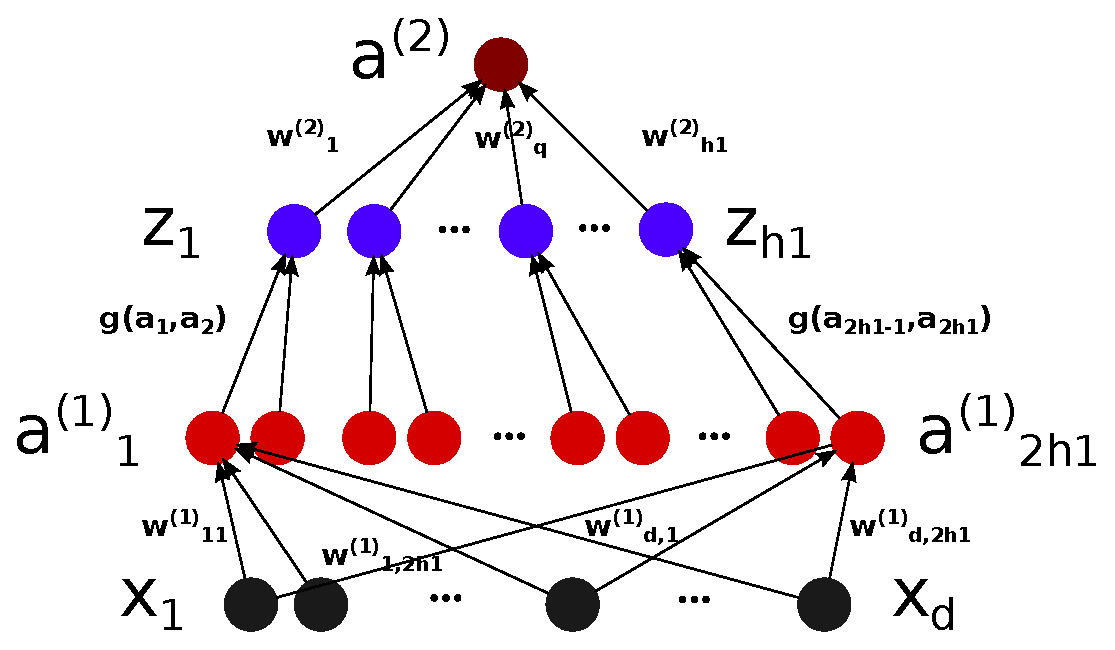
\includegraphics[width=.8\textwidth]{mlp/mlp.eps}
	\label{mlp}
	\caption{Schema of the MLP as described in the project instructions}
\end{figure}
\newline
\paragraph{Early stopping}
Evaluate empirical error $\hat{R}(\hat{f};\mathcal{D}_V)$ for validation set $\mathcal{D}_V$ along-side the training-error $\hat{R}(\hat{f};\mathcal{D}_T)$while training the MLP on $\mathcal{D}_T$. Stop at the training at the epoch where the validation error stops decreasing and starts increasing. 
\newline
Justify design and parameter choices\\
Show comparative plots illustrating the effects of learning rate, number of hidden units, momentum, etc. on\\

\paragraph{Effects of parameters on convergence speed}
\textsc{classifiers not tested on test set, only on validation set}

\begin{itemize}

	\item effects of the learning rate $\eta$\\
		\begin{figure}[!ht]
		\centering
		\begin{subfigure}[b]{.45\textwidth}
		\centering
		
\includegraphics[width=\textwidth]{mlp/placeholder.png}
		\caption{example subcaption}
		\end{subfigure}
		\quad
		\begin{subfigure}[b]{.45\textwidth}
		\centering
		
\includegraphics[width=\textwidth]{mlp/placeholder.png}
		\caption{example subcaption}
		\label{fig:subfigure2}
		\end{subfigure}
		\begin{subfigure}[b]{.45\textwidth}
		\centering
		
\includegraphics[width=\textwidth]{mlp/placeholder.png}
		\caption{example subcaption}
		\label{fig:subfigure3}
		\end{subfigure}
		\quad
		\begin{subfigure}[b]{.45\textwidth}
		\centering
		
\includegraphics[width=\textwidth]{mlp/placeholder.png}
		\caption{example subcaption}
		\label{fig:subfigure4}
		\end{subfigure}
		\caption{Example caption}
		\label{fig:example}
		\end{figure}

	\item Effects of number hidden units $h_1$
		\begin{figure}[!ht]
		\centering
		\begin{subfigure}[b]{.45\textwidth}
		\centering
		
\includegraphics[width=\textwidth]{mlp/placeholder.png}
		\caption{example subcaption}
		\end{subfigure}
		\quad
		\begin{subfigure}[b]{.45\textwidth}
		\centering
		
\includegraphics[width=\textwidth]{mlp/placeholder.png}
		\caption{example subcaption}
		\label{fig:subfigure2}
		\end{subfigure}
		\caption{Example caption}
		\label{fig:example}
		\end{figure}

	\item Effects of the momentum term	
		\begin{figure}[!ht]
		\centering
		\begin{subfigure}[b]{.45\textwidth}
		\centering
		
\includegraphics[width=\textwidth]{mlp/placeholder.png}
		\caption{example subcaption}
		\end{subfigure}
		\quad
		\begin{subfigure}[b]{.45\textwidth}
		\centering
		
\includegraphics[width=\textwidth]{mlp/placeholder.png}
		\caption{example subcaption}
		\label{fig:subfigure2}
		\end{subfigure}
		\caption{Example caption}
		\label{fig:example}
		\end{figure}

\end{itemize}

\subsubsection{Effects of parameter choice on overfitting}
show for which parameters training error decreases while validation increases
	\begin{figure}[!ht]
	\centering
	\begin{subfigure}[b]{.45\textwidth}
	\centering
	
\includegraphics[width=\textwidth]{mlp/placeholder.png}
	\caption{example subcaption}
	\end{subfigure}
	\quad
	\begin{subfigure}[b]{.45\textwidth}
	\centering
	
\includegraphics[width=\textwidth]{mlp/placeholder.png}
	\caption{example subcaption}
	\label{fig:subfigure2}
	\end{subfigure}
	\caption{Example caption}
	\label{fig:example}
	\end{figure}

include \textsc{typical} example of overfitting by letting the validation error increase while the training error decreases for a few, say 3, rounds!

\subsubsection{Determining parameters for binary subtasks}

\begin{figure}[!ht]
	\centering
		\begin{subfigure}[b]{.45\textwidth}
		\centering
		
\includegraphics[width=\textwidth]{mlp/placeholder.png}
		\caption{example subcaption}
		\end{subfigure}
	\quad
	\begin{subfigure}[b]{.45\textwidth}
	\centering
	
\includegraphics[width=\textwidth]{mlp/placeholder.png}
	\caption{example subcaption}
	\label{fig:subfigure2}
	\end{subfigure}
	\begin{subfigure}[b]{.45\textwidth}
	\centering
	
\includegraphics[width=\textwidth]{mlp/placeholder.png}
	\caption{example subcaption}
	\end{subfigure}
	\quad
	\begin{subfigure}[b]{.45\textwidth}
	\centering
	
\includegraphics[width=\textwidth]{mlp/placeholder.png}
	\caption{example subcaption}
	\label{fig:subfigure2}
	\end{subfigure}
	\caption{Example caption}
	\label{fig:example}
\end{figure}

\textsc{Comment on findings \textbf{qualitatively}}		

\section{Results}
	plots annotated by the result of the final classifier on the test set
	\subsection{Discussion of performance on test set}

	\subsection{Misclassified patterns}